% Indicate the main file. Must go at the beginning of the file.
% !TEX root = ../main.tex

%%%%%%%%%%%%%%%%%%%%%%%%%%%%%%%%%%%%%%%%%%%%%%%%%%%%%%%%%%%%%%%%%%%%%%%%%%%%%%%%
% 04_discussion
%%%%%%%%%%%%%%%%%%%%%%%%%%%%%%%%%%%%%%%%%%%%%%%%%%%%%%%%%%%%%%%%%%%%%%%%%%%%%%%%


\section{Discussion}
\label{discussion}

\subsection{Best Model Performance}

The best performing model achieved a reasonable high accuracy of 0.92. The validation
metrics loss and accuracy are shown in \autoref{fig:best_model_training_metrics}
suggest a reasonable progress during the fitting process. Since they both are not
all the way flattening out, it might even be possible to further improve the model
using the same architecture and hyperparameters by training it for more epochs.
This could be achieved by using a higher value for the \texttt{patience} parameter --
the next value to be tested could be 20 instead of 10.

\begin{figure}[H]
    \centering
    \captionsetup{width=0.8\linewidth}
    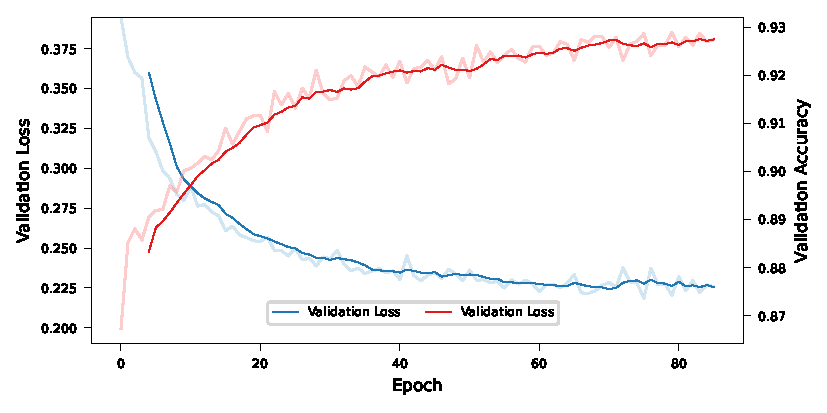
\includegraphics{figures/best_model_training_metrics.pdf}
    \caption{Validation loss and accuracy for the best model.}
    \label{fig:best_model_training_metrics}
\end{figure}

The accuracy per class, shown in \autoref{fig:best_model_accuracy_per_category}
does align with expectations. Classes like \texttt{Building}, \texttt{GreenAreas}, \texttt{RoadAsphalt}, \texttt{Forrest},
and \texttt{MadowPasture} are predicted with high accuracy. While classes, where there is
very little data available like \texttt{WaterBasin} or classes where the data is more vague
like \texttt{ConstructionSites} are predicted with lower accuracy.

From the visual inspection of the predictions in \autoref{fig:best_model_predictions},
it looks like the borders between the classes are difficult to predict. This can be
explained by the fact that the classes are not always very precise and this would
specifically effect this areas. An other explanation could be the resolution of 10cm
which leads to pixel in reality consisting of multiple classes -- this issue referred to
as mixed pixels -- could be the part of the reason for the lower accuracy in the
border areas.

\subsection{Hyperparameter Tuning}

The hyperparameter tuning process was successful in finding the best hyperparameters
within the grid search. From \autoref{fig:hp_tuning_boxplot} it can be seen that
lower values for the \texttt{learning\_rate} seem to work better and that
a higher regulation during training -- a higher value \texttt{weight\_decay} -- leads to
better results. Very interesting is the fact that the benefit of the data augmentation
seems to correlate with more regularization during training.
The grid of evaluated hyperparameters was rather limited dew to limited computational
resources in the remaining time. A more extensive search could potentially lead to
even better results. What might really be worth trying is to test for even smaller
values of \texttt{learning\_rate}, higher values for \texttt{weight\_decay} 
and to use the other options for the data augmentation --
pixel- and channel noise in different combinations.

\subsection{Comparing the Results to the GIS Approach}

Since the validation for the original studies was done for a different are in Rünenberg,
using a different dataset, it is hard to compare the results directly. Adding to that,
different land cover categories where used and different resolutions. Over all, the
original studies achieved an accuracy of 0.9 to 1 for the more obvious classes like
\texttt{Buildings}, \texttt{SealedRoads}, \texttt{GreenAreas} and \texttt{MadowPastures}. 
For the more difficult classes like \texttt{PathUnsealed} and \texttt{SealedObjects} the
accuracy was lower as well. The results of this study -- as different they are created --
reach a similar range of accuracy.

\subsection{Prospects}

The results of this study show that the approach of using deep learning for perviousness
classification is promising. The results are in a similar range as the results of the
original study using a GIS approach. Therefore it might be worth to further investigate
the potential of deep learning for this task. The next steps besides the mentioned hyperparameter
expansion, more data augmentation and more thorough training going for more epochs there are other
promising approaches. One could be to try different model concept like U-Net -- specifically
designed for image segmentation tasks. Another approach could be to use a pre-trained model
to build upon -- there the issue is to find a model that is trained on similar data and
accepts four channels as input. An other idea could be to implement some self supervised
learning techniques utilizing not labeled data to improve the model. As for most of the deep
learning tasks, the more data the better -- so it would be worth to try to get more data
of a possibly even higher quality to improve the existing models.